\chapter{Introdução}

\section{História da Genética}

\indent O estudo do núcleo celular começou no século XIX com o objetivo de <<<<<<>>>>>>.  pesquisa era do bioquímico suíço Friedrich Miescher, <<<<<<>>>>>>. Duas teorias divergetes marcaram esta época: enquanto Charles Darwin afirmava que a evolução era um evento demorado e o ser <<<<<<>>>>>>sobrevivente<<<<<<>>>>>> era escolhido aleatoriamente, Gregor Mendel insistia que a evolução acontecia a cada geração e, ainda, podia ser controlada. Foi apenas nas pesquisas do grupo de Thomas Morgan que essas duas teorias vieram a se <<<<<<>>>>>>unir<<<<<<>>>>>>.

A partir do século XX, o foco passou a ser a compreensão da produção de proteínas nos seres vivos e, para isso, <<<<<<>>>>>>.

\indent A linha do tempo abaixo tem o objetivo de auxiliar na localização temporal da história da biologia molecular ao passo que apresentam as datas de nascimento e morte dos principais pesquisadores da área, cujos trabalhos serão descritos neste capítulo. 

%  -------------------------------------------- 
%  -------------------------------------------- LINHA DO TEMPO
%  -------------------------------------------- 

\begin{timeline}{1809}{2004}{2cm}{2.5cm}{15cm}{24cm}
\entry{1809}{$\star$ Charles Darwin, PAÍS}
\entry{1822}{$\star$ Gregor Mendel, PAÍS}
\entry{1844}{$\star$ Friedrich Miescher, PAÍS}
\entry{1859}{Darwin publica livro A Origem das Espécies} %On the Origin of Species by Means of Natural Selection,
% or the Preservation of Favoured Races in the Struggle for Life.
%  6º ed. It is in this edition that the word 'evolution' occurs for the first time.
% http://darwin-online.org.uk/content/frameset?pageseq=80&itemID=A1&viewtype=text
% Genes sobreviventes demoram a se espalhar pois são aleatóriamente selecionados
\entry{1865}{Mendel apresenta pela primeira vez seu trabalho com ervilhas} % após 8 anos de experimentos (1856-1863)
% na Nature Research Society of Brünn: The Law of Segregation and The Law of Independent Assortment.
% http://www.wired.com/2010/02/0208gregor-mendel-reads-paper/
% Dominante, recessivo, hereditariedade. Características passadas independentemente
\entry{1866}{$\star$ Thomas Morgan, PAÍS}
\entry{1871}{Miescher ---------------- núcleo celular}
\entry{1882}{$\dagger$ Charles Darwin}
\entry{1884}{$\dagger$ Gregor Mendel}
\entry{1890}{$\star$ Hermann Muller, PAÍS}
\entry{1895}{$\dagger$ Friedrich Miescher} %%
\entry{1916}{$\star$ Francis Crick, PAÍS}
\entry{1928}{$\star$ James Watson, PAÍS}
\entry{1945}{$\dagger$ Thomas Morgan}
\entry{1967}{$\dagger$ Hermann Muller}
\entry{2004}{$\dagger$ Francis Crick}
\end{timeline}

%  -------------------------------------------- 
%  -------------------------------------------- LINHA DO TEMPO
%  -------------------------------------------- 


\subsection{Origens da Vida}

\indent ...

\subsection{Análise do Núcleo Celular}

\indent ...

\vspace{1cm}
 \begin{figure}[h!]
     \centering
     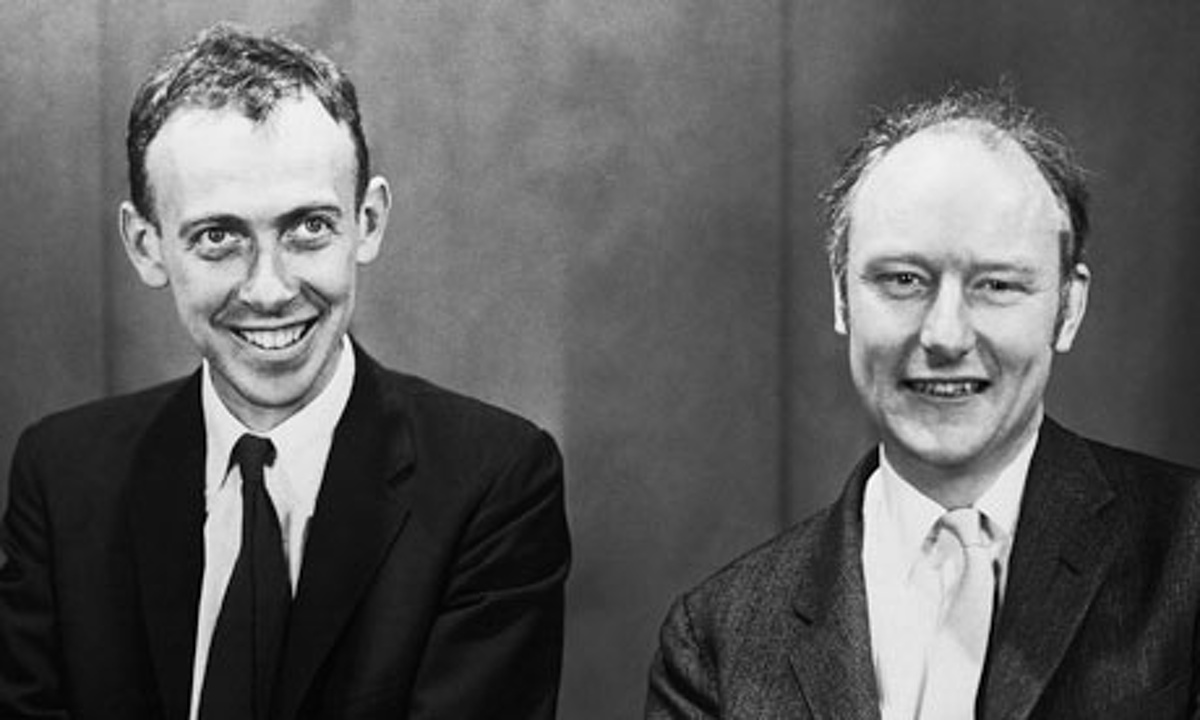
\includegraphics[scale=0.4]{JamesWatsonAndFrancisCrick.jpg}
     \caption{Pai da bio}
     \label{fig:JamesWatsonAndFrancisCrick}
 \end{figure}
\vspace{1cm}

\subsection{Estudo do genoma}

\indent ... 



%  -------------------------------------------------------------
%  -------------------------------------------------------------

\section{Sequenciamento genético}

\indent ...

%  -------------------------------------------------------------
%  -------------------------------------------------------------

\section{Definição do Problema}

\indent 
Contruir uma visualização interativa de redes metabólicas aramazenadas em \textit{Graph Databases} que permita ao pesquisador explorar os aspectos biológicos do organismo estudado.



\section{Justificativa}

\indent 
% Falar da quantidade de dados que e muito grande para ser examinada e o quanto um sistema com busca e uma visualizacao interativa
% pode auxiliar o pesquisador.

Atualmente, a quantidade de dados <<<<>>>> estudados pelos pesquisadores é extensa e complexa. Uma maneira de amenizar o esforço feito para analisar os dados e compreendê-los é oferecer uma ferramenta que aproxime o usuário (pesquisador) e os dados em forma de grafo(redes metabólicas). Esta ferramenta deverá permitir que o usuário visualize e interaja com os dados dinamicamente, além de disponibilizar mecanismos de busca em grafos, úteis para sua pesquisa.


\section{Objetivo}

\indent 
Constrir um sistema que acesse redes metabólicas armazenadas em bancos de dados em grafo e gere uma visualização interativa
\begin{itemize}
 \item Implementar uma busca das vias metabólicas de interesse a apartir de parâmetros informados pelo pesquisador no sistema
 \item Recuperar a informação desejada e exibí-la para o pesquisador de forma ergonômica
 \item Implementar algoritmos de busca em grafos para recuperar a informação solicitada e/ou sugerir informação relevante
\end{itemize}

\section{Descrição dos Capítulos}

\indent No Capítulo 1 fez-se uma breve introdução aos ... No Capítulo 2 são estabelecidas as principais definições utilizadas neste trabalho mais profundamente, tais 
como ... Ainda, são apresentados ... Também são descritos ... O Capítulo 3 faz referência à implementação do... 






